\documentclass[a4paper,11pt]{article}

\usepackage[left=2.5cm,right=2.5cm,top=3cm,bottom=3cm,pdftex]{geometry}
\usepackage{amssymb, amsmath, url, natbib, float, subcaption, listings,mathtools, physics}
\usepackage[utf8]{inputenc}
\usepackage[T1]{fontenc}
\renewcommand{\topfraction}{0.9}
\lstset{basicstyle=\scriptsize\tt,}
\usepackage[pdftex]{graphicx}
\pdfcompresslevel=9 
\DeclareGraphicsExtensions{.png, .pdf, .jpg}
\usepackage[pdftex, colorlinks, linkcolor=blue, urlcolor=blue, citecolor=blue, pagecolor=blue, breaklinks=true]{hyperref}
\usepackage{tikz}

\begin{document}
\pagestyle{empty}
\title{Pursuit Models}
\section{Introduction}
We consider the setup where a player is running and another player is chasing the runner inside the court. We assume that the goal of the chaser is to get in the vicinity of the runner and thus the chaser is running towards the current position of the runner. The current spatial coordinates of the runner is $(x^{r}, y^{r})$ and those of the chaser is $(x^{c}, y^{c})$. Since the chaser is moving towards the runner, the velocity vector of the chaser is pointed towards the runner's current position.

\begin{figure}[H]
\centering
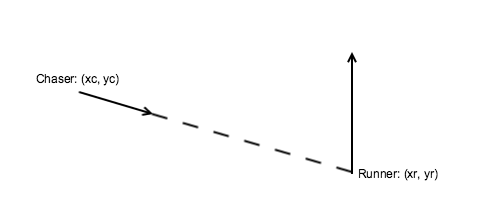
\includegraphics[width=0.8\textwidth]{pursuit.png}
\caption{Paths for runner and chaser}
\end{figure}

The velocity of the chaser, $(\dot{x}^c, \dot{y}^c)$, can thus be given as
\begin{align*}
(\dot{x}^c, \dot{y}^c) = \gamma(t) (x^{r} - x^{c}, y^{r} - y^{c})
\end{align*}

where the velocity vector of the chaser is $\vec{\phi} = (x^{r} - x^{c}, y^{r} - y^{c})$ and the speed of the chaser is $\gamma(t)$. If we know the runner's position at different time points, the system of ODEs for the chaser is as follows,

\begin{align*}
d(x^{c}, y^{c}) & = \gamma(t) \frac{\vec{\phi}}{||\vec{\phi}||} dt + (\nu_1 dW^1_t, \nu_2 dW^2_t) \\
\implies d x^{c} & = \frac{\gamma(t) (x^{r} - x^{c})}{\sqrt{(x^{r} - x^{c})^2 + (y^{r} - y^{c})^2}}dt + \nu_1 dW^1_t \\
d y^{c} & = \frac{\gamma(t) (y^{r} - y^{c})}{\sqrt{(x^{r} - x^{c})^2 + (y^{r} - y^{c})^2}}dt + \nu_2 dW^2_t
\end{align*}

The Euler-Maruyama approximation of the above system of ODEs is

\begin{align*}
x^{c}_{i+1} & = x^{c}_{i} + \frac{\gamma(t) (x^{r}_{i} - x^{c}_{i})}{\sqrt{(x^{r}_{i} - x^{c}_{i})^2 + (y^{r}_{i} - y^{c}_{i})^2}} h + \nu_1 \sqrt{h} Z_1 \\
y^{c}_{i+1} & = y^{c}_{i} + \frac{\gamma(t) (y^{r}_{i} - y^{c}_{i})}{\sqrt{(x^{r}_{i} - x^{c}_{i})^2 + (y^{r}_{i} - y^{c}_{i})^2}}h + \nu_2 \sqrt{h} Z_2
\end{align*}
Some examples of  \href{http://home2.fvcc.edu/~dhicketh/DiffEqns/Spring11projects/Jonah_Franchi_Katy_Steiner/Diff%20EQ%20Project.pdf}{Pursuit Curves} and proofs of the trajectory for different models considered.

\section{Numerical Method}
We consider the coupled SDE model:

\begin{subequations}
\begin{equation}
d X_{1,t} = f_{1} (t, \mathbf{X}_t, \theta) dt + g_{1} (t, \mathbf{X}_t, \theta) dW_{1,t}
\end{equation}    
\begin{equation}
d X_{2,t} = f_{2} (t, \mathbf{X}_t, \theta) dt + g_{2} (t, \mathbf{X}_t, \theta) dW_{2,t}
\end{equation}
\end{subequations}
$f_1, f_2$ represent the drift functions and $g_1, g_2$ are the diffuction functions. $\mathbf{X}_t = (X_{1,t}, X_{2,t})$ and $W_{1,t}, W_{2,t}$ are two independent Wiener processes. \\

We discretize the SDE using Euler-Maruyama approximation
\begin{subequations}
\begin{equation}
X_{1}^{n+1} = X^n_1 + f_{1} (t_n, \mathbf{X}^{n}, \theta) h + g_{1} (t_n, \mathbf{X}^n, \theta) \sqrt{h} Z^{n+1}_1
\end{equation}    
\begin{equation}
X_{2}^{n+1} = X^n_2 + f_{2} (t_n, \mathbf{X}^{n}, \theta) h + g_{2} (tn, \mathbf{X}^n, \theta) \sqrt{h} Z^{n+1}_2
\end{equation}
\end{subequations}

The main goal is to compute the likelihood $p(\vec{x} | \theta)$. Using Markov property and approximating the full probability by discrete transition probability, $p(x_{m+1} | p(x_m), \theta)$, this can be approximated as
$$
p(\vec{x} | \theta) \approx \sum_{m=0}^{M-1} \tilde{p}(x_{m+1} | x_m , \theta)
$$

\begin{equation}
\tilde{p}^{n+1} (x_1, x_2 | \theta) = \int_{y_1, y_2 \in \mathbb{R}^2} \mathbb{K}^{n}(x_1, x_2, y_1, y_2, t_n; \theta) \tilde{p}^n (y_1, y_2, t_n | \theta) dy
\end{equation}

where $\mathbb{K}^{n}(x_1, x_2, y_1, y_2, t_n; \theta) = \tilde{p}^{n+1 | n} (x_1, x_2 | y_1, y_2, t_n; \theta) = \frac{1}{\sqrt{2 \pi \sigma_1^2}} \exp \frac{-(x_1 - \mu_1)^2}{2\sigma^2_1} \frac{1}{\sqrt{2 \pi \sigma_2^2}} \exp \frac{-(x_2 - \mu_2)^2}{2\sigma^2_2}$ given
$\mu_1 = y_1 + f_1 (y_1, y_2, t_n ; \theta) h, \mu_2 = y_2 + f_2 (y_1, y_2, t_n ; \theta) h, \sigma_1^2 = g^2_1(y_1, y_2, t_n ; \theta) h, \sigma_2^2 = g^2_2 (y_1, y_2, t_n ; \theta) h$ \\

Once we have a numerical method setup, we create the 2D spatial grid, $-M \leq x \leq M, -M \leq y \leq M$. For the purpose of numerical integration, $x_1^i = ik, x_2^j = jk, y_1^{i'} = i'k, y_2^{j'} = j'k$. Applying the trapezoidal rule on both the variables $y_1$ and $y_2$,

\begin{equation}
\hat{p}^{n+1}(x_1^{i}, x_2^{j}; \theta) = k^2 \sum_{i' = -\infty}^{\infty} \sum_{j' = -\infty}^{\infty} \mathbb{K}^{n}(x_1^{i}, x_2{j}, y_1^{i'}, y_2^{j'}; \theta) \hat{p}^{n}(y_1^{i'}, y_2^{j'}; \theta)  
\end{equation}

Rather than summing over all of $\mathcal{R}^2$, we sum over windows of $\gamma = \frac{2 \sqrt{h} \sup{g}}{k}$.

\begin{equation}
\hat{p}^{n+1}(x_1^{i}, x_2^{j}; \theta) = k^2 \sum_{i' = i-\gamma}^{i+\gamma} \sum_{j' = j-\gamma}^{j+\gamma} \mathbb{K}^{n}(x_1^{i}, x_2{j}, y_1^{i'}, y_2^{j'}; \theta) \hat{p}^{n}(y_1^{i'}, y_2^{j'}; \theta)  
\end{equation}

We start the process from a deterministic initial condition, $\mathbf{X}^0 = \mathbf{x}_m$ for each time interval $ (t_m, t_{m+1})$. This corresponds to the delta distribution at the initial condition, $\tilde{p}^0(x) = \delta(\mathbf{x} - \mathbf{x}_m)$. We thus compute the first step manually to obtain a Gaussian density for $\tilde{p}^{1}(x)$. 

// Talk about the interpolation, last step.

\section{Simulations}
For the purposes of simulation, the 2D grid considered is of the size of the standard basketball court, 94 ft. $\times$ 50 ft.  \\

The first simulation creates the runner's trajectory as $y^{r} = 5\log(x^{r})$. The chaser's speed is $\gamma(t) = 1+2t$ and we consider 10 points along the trajectory.

\begin{figure}[H]
\centering
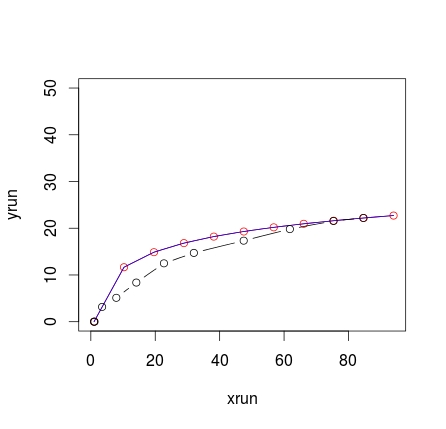
\includegraphics[width=0.7\textwidth]{simulation.jpeg}
\caption{Runner (red), Chaser (black) simulation for well-defined runner trajectory}
\end{figure}

For the second simulation, we consider 50 points on both the trajectories. The runner's trajectory in this case is randomized. $y^{r} = ((x^{r})^2)/100 + (x^{r}/20) + \mathcal{N}(\mu = 0, \sigma = 2)$.
\begin{figure}[H]
\centering
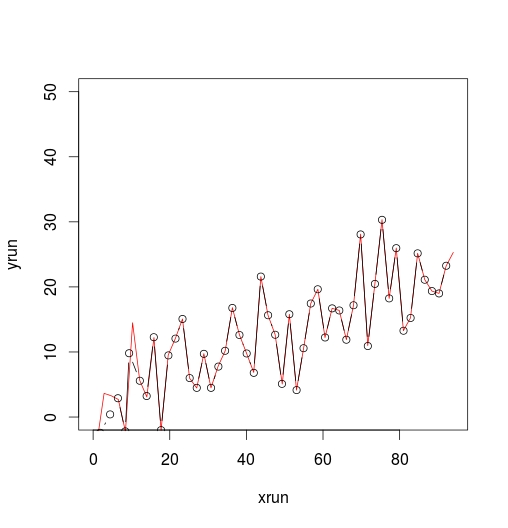
\includegraphics[width=0.8\textwidth]{sim50points.jpeg}
\caption{Simulation with random runner movement, time proportional speed of the chaser}
\end{figure}

In the third simulation, we take the speed of the chaser constant (upto some noise), $y^{c} = $
\begin{figure}[H]
\centering
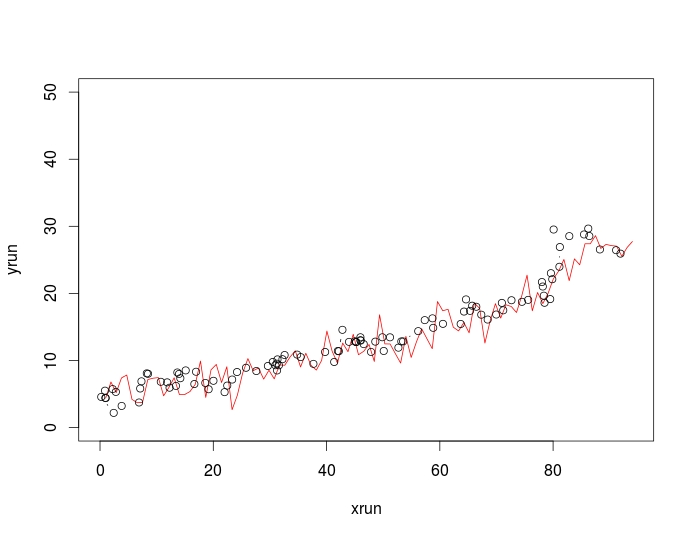
\includegraphics[width=0.8\textwidth]{sim100points_randomizedtraj.jpeg}
\caption{Simulation with constant speed (upto some noise) of the chaser}
\end{figure}


\section{Test 1:}
$\Delta t = 0.4, h = 0.4, numsteps = 1, k = 0.5, (x_{max}, y_{max}) = (5,5), \gamma(t) = (1,1), \nu_1 = 0.5, \nu_2 = 0.5$ \\

True value used for generating the fake data: $\gamma = (1.2, 1.2), \nu_1 = 0.5, \nu_2 = 0.5$
\begin{table}[H]
\centering
\begin{tabular}{|c|c|c|}
\hline
Time   & Runner & Chaser \\ \hline
$t_1$ = 0.0 & (1, 1.89)  & (0.54, 0.36)  \\ \hline
$t_2$ = 0.4 & (5, 1.05) &  (0.17, 0.96) \\ \hline
\end{tabular}
\end{table}

Starting values $(\gamma(t_1), \gamma(t_2), \nu_1, \nu_2) = (1, 1, 0.5, 0.5)$
\begin{table}[H]
\centering
\begin{tabular}{|c|c||c|c||c|c||c|c|}
\hline
$\gamma(t_1)$ & Posterior & $\gamma(t_2)$ & Posterior & $\nu_1$ & Posterior & $\nu_2$ & Posterior \\ \hline
& & 0 & -22.92144 & & & & \\ \hline
0.2 & -23.71904 & 0.2 & -22.92144 & 0.1 & -24.58937 & 0.1 & -29.03891 \\ \hline
0.4 & -23.45817 & 0.4 & -22.92145 & 0.2 & -22.89126 & 0.2 & -23.69771 \\ \hline
0.6 & -23.23481 & 0.6 & -22.92146 & 0.3 & -22.8476 & 0.3 & -22.98391 \\ \hline
0.8 & -23.05432 & 0.8 & -22.92147 & 0.4 & -22.91301 & 0.4 & -22.87974 \\ \hline
1 &  -22.92149  & 1 & -22.92149 & 0.5 & -22.92149 & 0.5 & -22.92149 \\ \hline
1.2 & -22.84025 & 1.2 & -22.92151 & 0.6 & -22.90837 & 0.6 & -23.00528 \\ \hline
1.4 & -22.81369 & 1.4 & -22.92154 & 0.7 & -22.90559 & 0.7 & -23.10002 \\ \hline
1.6 & -22.84412 & 1.6 & -22.92157 & 0.8 & -22.91925 & 0.8 & -23.19499 \\ \hline
1.8 & -22.93326 & 1.8 & -22.9216 & 0.9 & -22.94629 & 0.9 & -23.28634 \\ \hline
2 & -23.08237 & 2 & -22.92164 & & & & \\ \hline
2.2 & -23.29237 & 2.2 & -22.92168 & & & & \\ \hline
2.4 & -23.5639 & 2.4 & -22.92173 & & & & \\ \hline
2.6 & -23.89746 & 2.6 & -22.92178 & & & & \\ \hline
\end{tabular}
\end{table}

\begin{figure}[H]
\centering
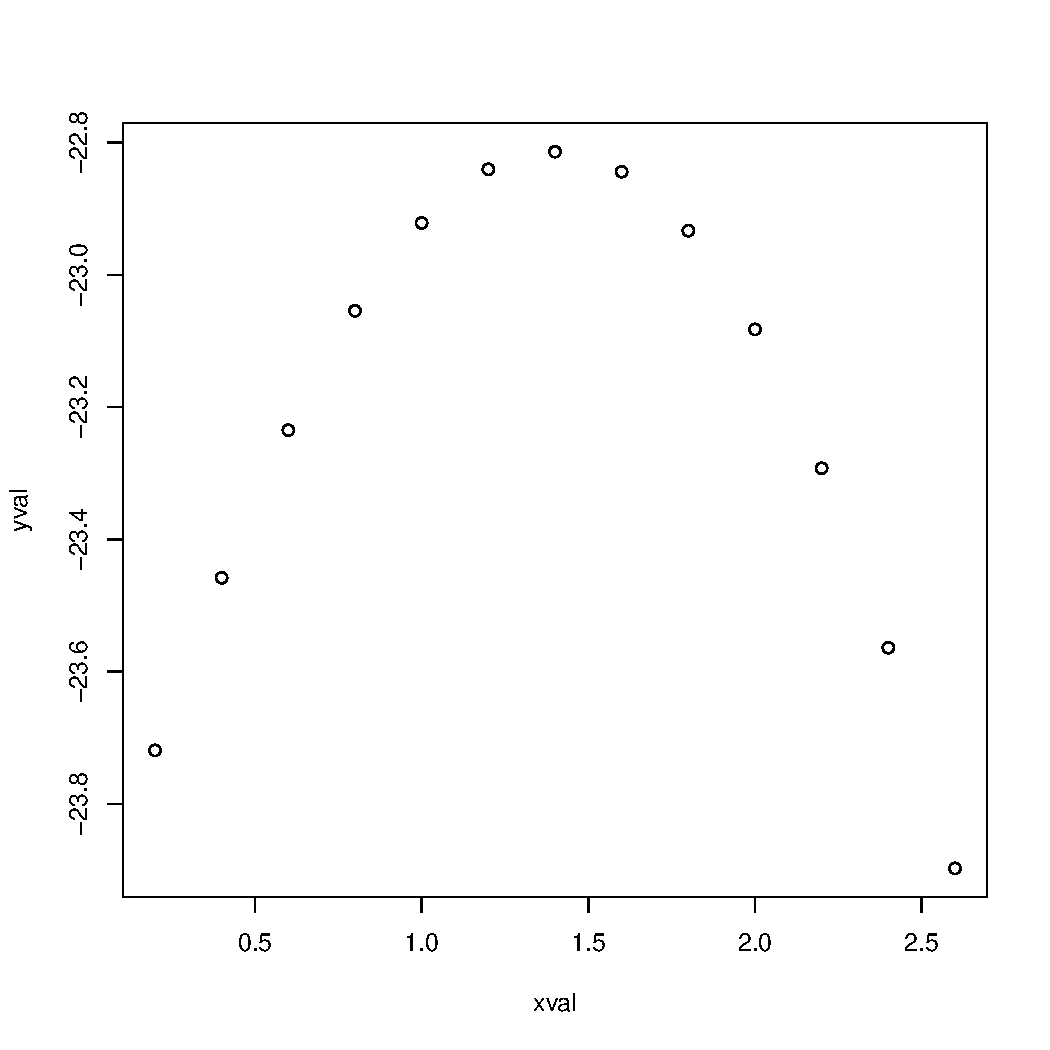
\includegraphics[width=0.8\textwidth]{test1_gamma1.pdf}
\caption{$\gamma(t_1)$ variations, ($\gamma(t_2) = 1, \nu_1 = 0.5, \nu_2 = 0.5$)}
\end{figure}

\begin{figure}[H]
\centering
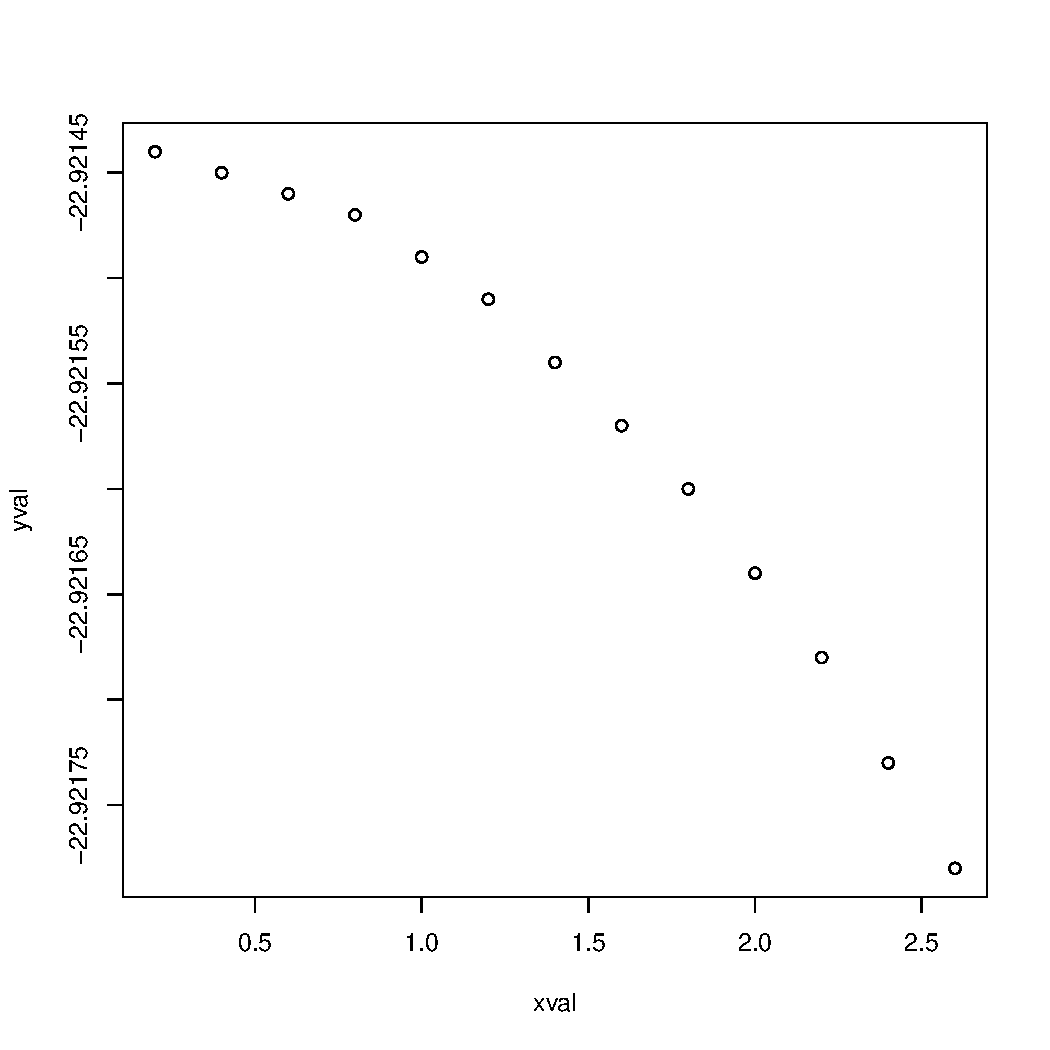
\includegraphics[width=0.8\textwidth]{test1_gamma2.pdf}
\caption{$\gamma(t_2)$ variations, ($\gamma(t_1) = 1, \nu_1 = 0.5, \nu_2 = 0.5$)}
\end{figure}

\begin{figure}[H]
\centering
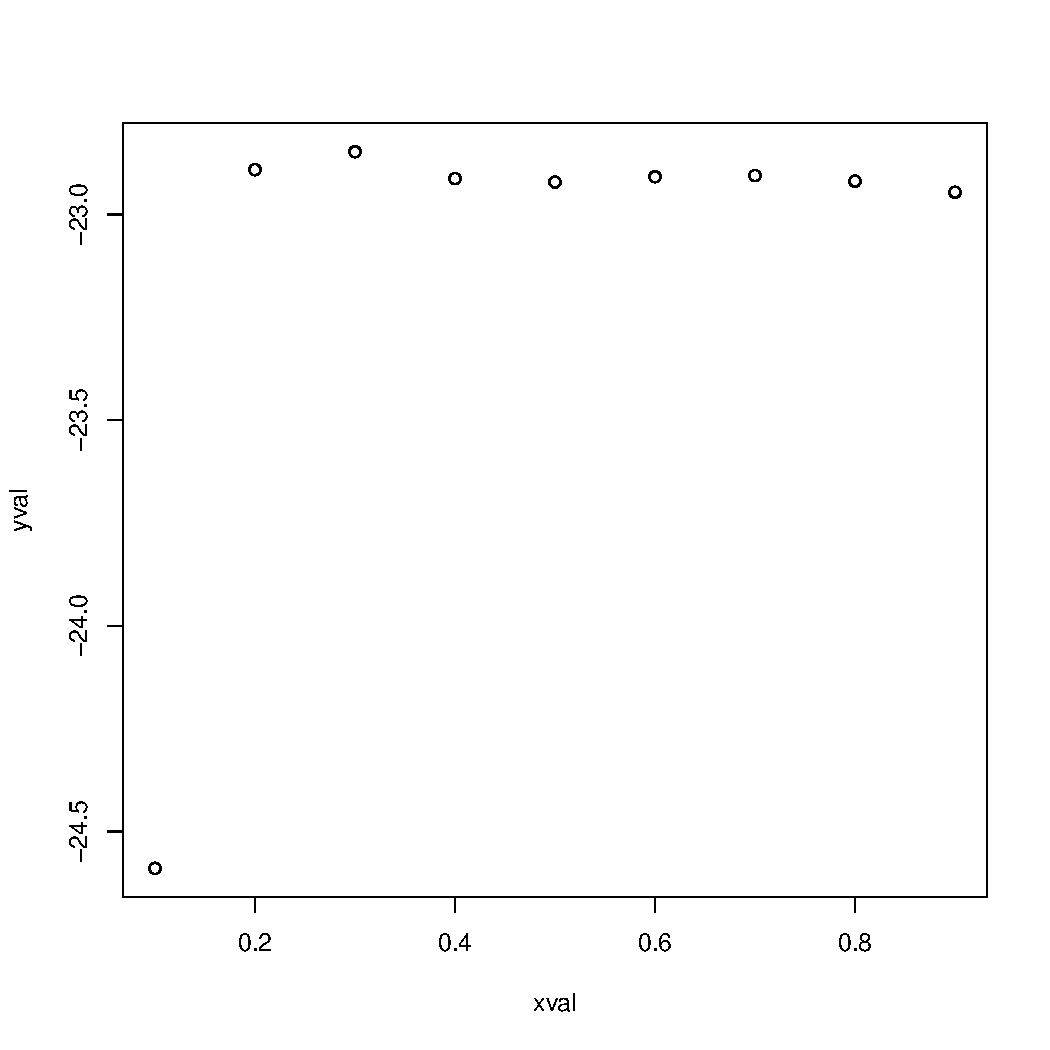
\includegraphics[width=0.8\textwidth]{test1_nu1.pdf}
\caption{$\nu_1$ variations, ($\gamma(t_1) = 1, \gamma(t_2) = 1, \nu_2 = 0.5$)}
\end{figure}

\begin{figure}[H]
\centering
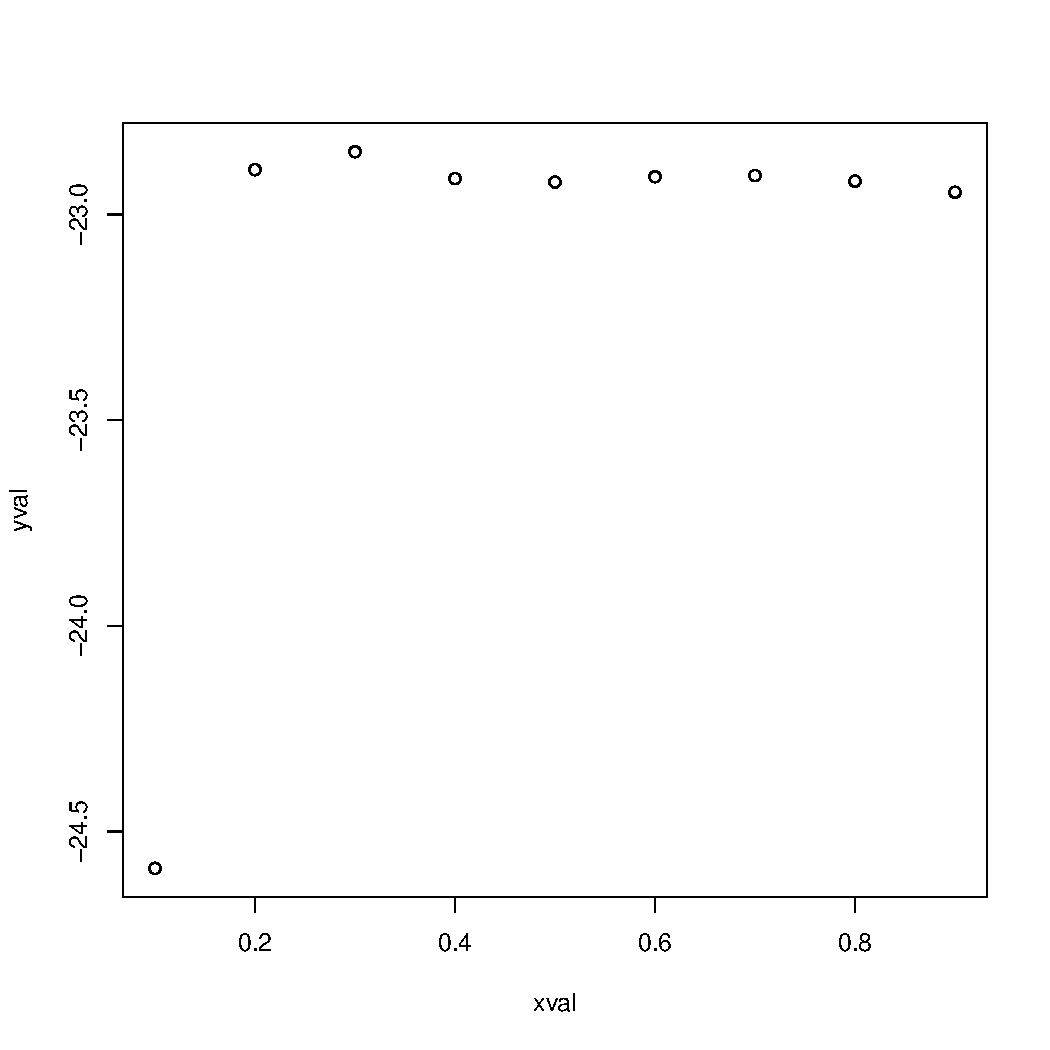
\includegraphics[width=0.8\textwidth]{test1_nu2.pdf}
\caption{$\nu_1$ variations, ($\gamma(t_1) = 1, \gamma(t_2) = 1, \nu_1 = 0.5$)}
\end{figure}



\section{Test 2:}
$\Delta t = 0.4, h = 0.2, numsteps = 2, k = 0.5, (x_{max}, y_{max}) = (5,5), \gamma(t) = (1,1), \nu_1 = 0.5, \nu_2 = 0.5$ \\

True value used for generating the fake data: $\gamma = (1.2, 1.2), \nu_1 = 0.5, \nu_2 = 0.5$
\begin{table}[H]
\centering
\begin{tabular}{|c|c|c|}
\hline
Time   & Runner & Chaser \\ \hline
$t_1$ = 0.0 & (1, 1.89)  & (0.54, 0.36)  \\ \hline
$t_2$ = 0.4 & (5, 1.05) &  (0.17, 0.96) \\ \hline
\end{tabular}
\end{table}

Starting values $(\gamma(t_1), \gamma(t_2), \nu_1, \nu_2) = (1, 1, 0.5, 0.5)$
\begin{table}[H]
\centering
\begin{tabular}{|c|c||c|c||c|c||c|c|}
\hline
$\gamma(t_1)$ & Posterior & $\gamma(t_2)$ & Posterior & $\nu_1$ & Posterior & $\nu_2$ & Posterior \\ \hline
0.2 & -23.83499 & 0.2 & -23.68217 & 0.1 & -31.66729 & 0.1 & -23.9696 \\ \hline
0.4 & -23.7425 & 0.4 & -23.68217 & 0.2 & -24.38675 & 0.2 & -23.8535 \\ \hline
0.6 & -23.6859 & 0.6 & -23.68218 & 0.3 & -23.58051 & 0.3 & -24.25005 \\ \hline
0.8 & -23.6657 & 0.8 & -23.6822 & 0.4 & -23.57827 & 0.4 & -24.00326 \\ \hline
1 &  -23.68221  & 1 & -23.68221 & 0.5 & -23.68221 & 0.5 & -23.68221 \\ \hline
1.2 & -23.73577 & 1.2 & -23.68224 & 0.6 & -23.71837 & 0.6 & -23.54345 \\ \hline
1.4 & -23.82691 & 1.4 & -23.68226 & 0.7 & -23.70203 & 0.7 & -23.52035 \\ \hline
1.6 & -23.95648 & 1.6 & -23.68229 & 0.8 & -23.68004 & 0.8 & -23.55228 \\ \hline
\end{tabular}
\end{table}

\begin{figure}[H]
\centering
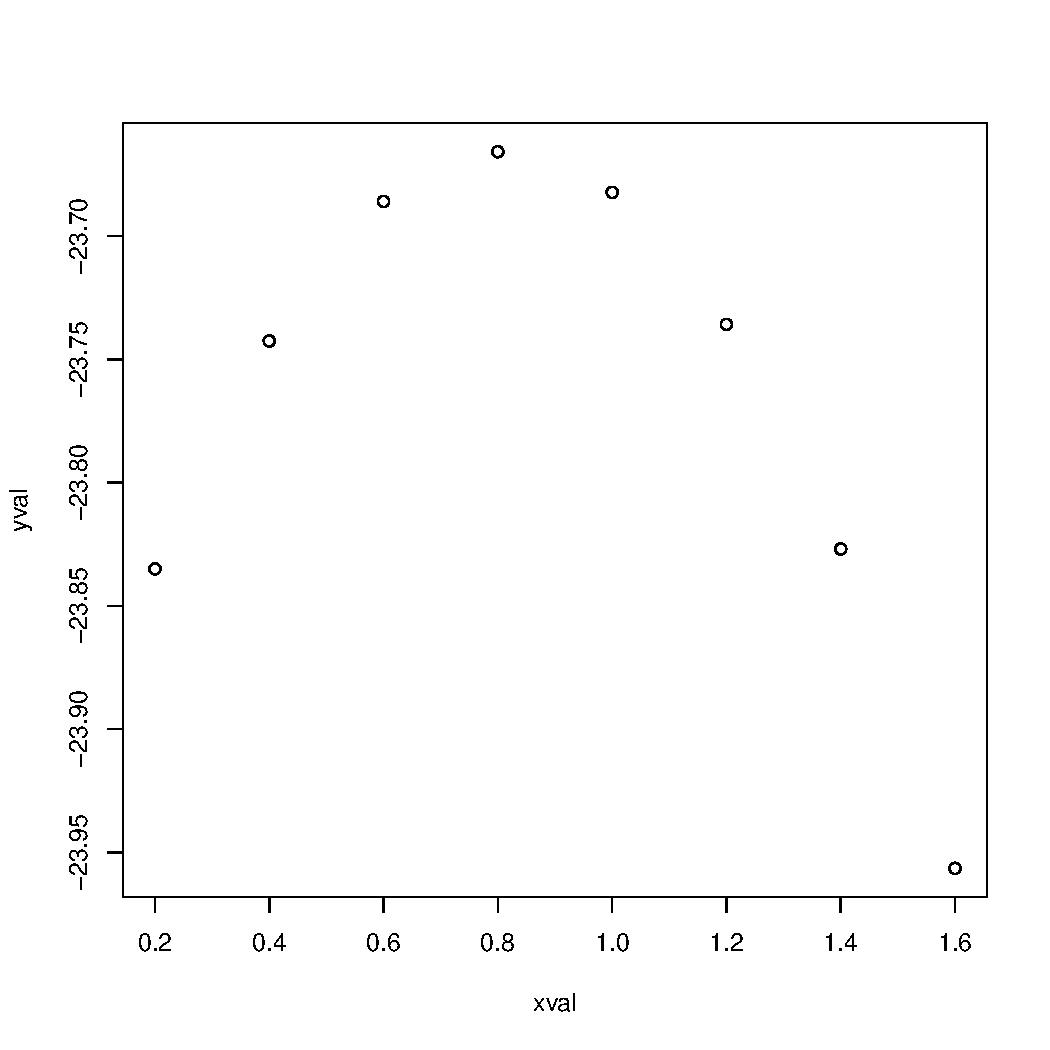
\includegraphics[width=0.8\textwidth]{test2_gamma1.pdf}
\caption{$\gamma(t_1)$ variations, ($\gamma(t_2) = 1, \nu_1 = 0.5, \nu_2 = 0.5$)}
\end{figure}

\begin{figure}[H]
\centering
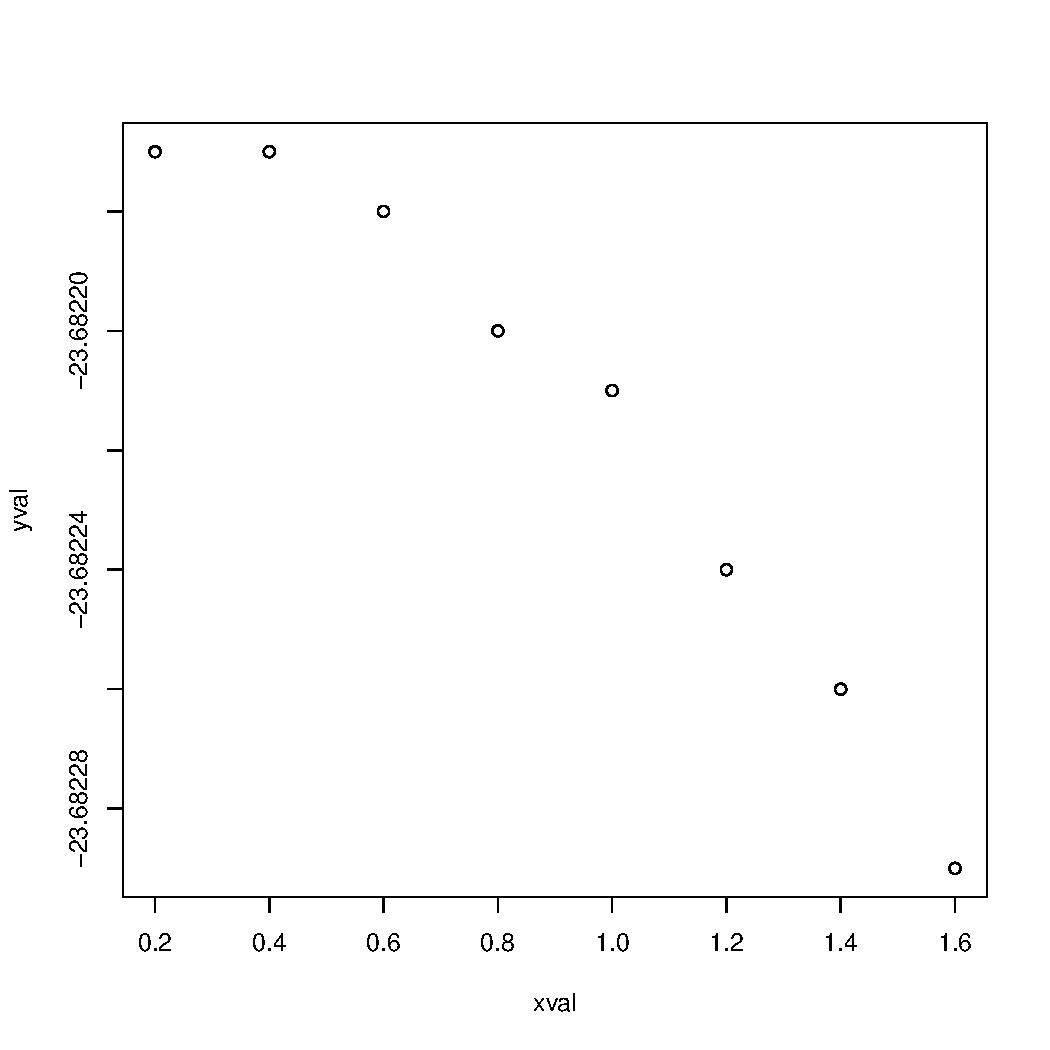
\includegraphics[width=0.8\textwidth]{test2_gamma2.pdf}
\caption{$\gamma(t_2)$ variations, ($\gamma(t_1) = 1, \nu_1 = 0.5, \nu_2 = 0.5$)}
\end{figure}

\begin{figure}[H]
\centering
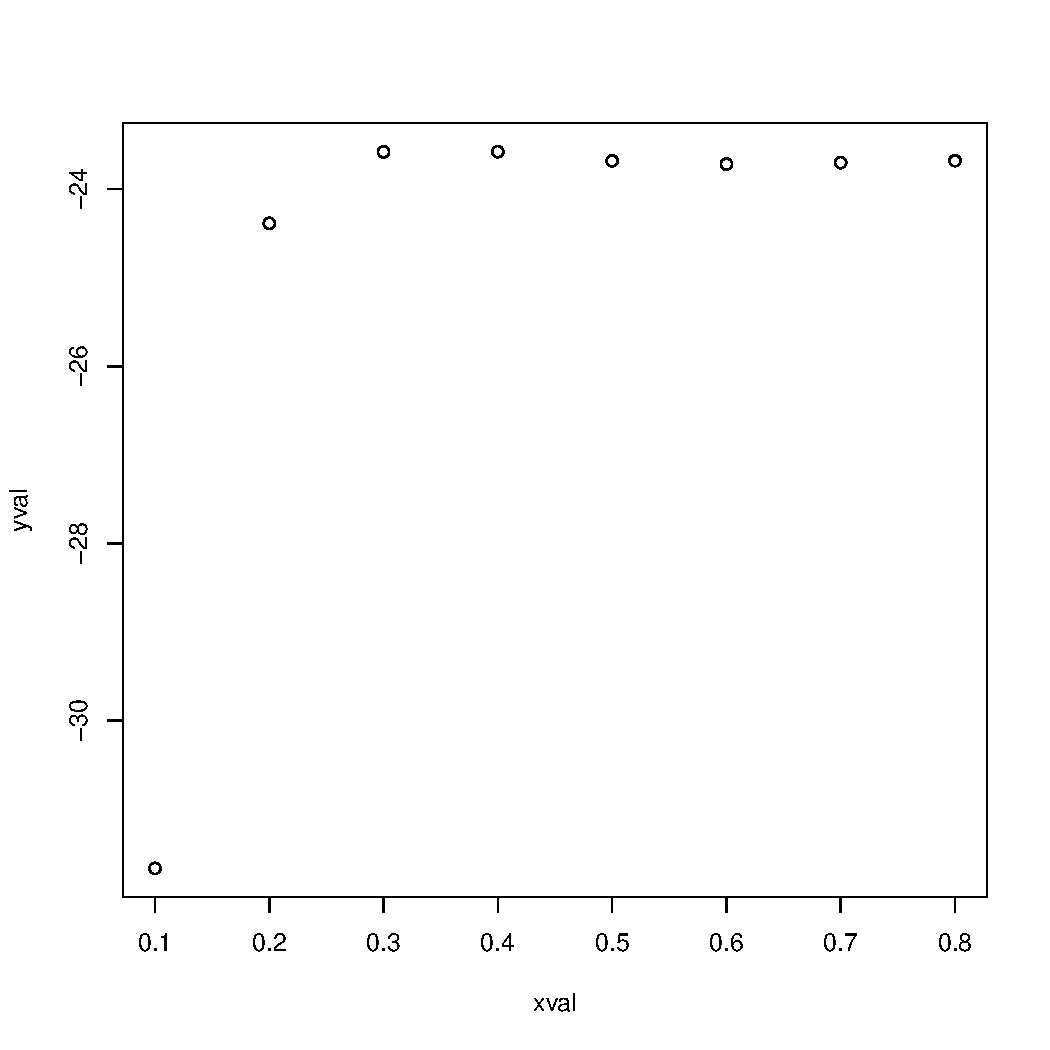
\includegraphics[width=0.8\textwidth]{test2_nu1.pdf}
\caption{$\nu_1$ variations, ($\gamma(t_1) = 1, \gamma(t_2) = 1, \nu_2 = 0.5$)}
\end{figure}

\begin{figure}[H]
\centering
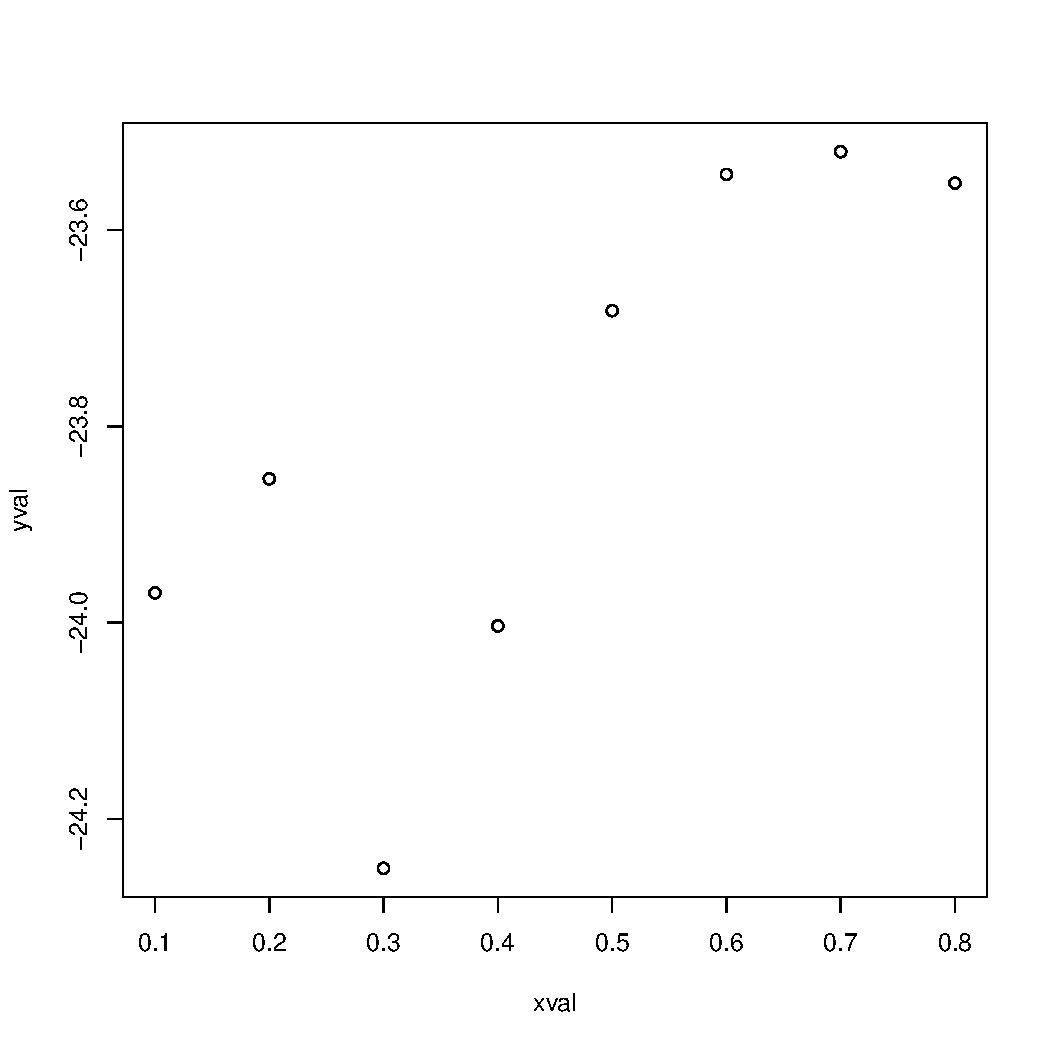
\includegraphics[width=0.8\textwidth]{test2_nu2.pdf}
\caption{$\nu_1$ variations, ($\gamma(t_1) = 1, \gamma(t_2) = 1, \nu_1 = 0.5$)}
\end{figure}

\section{Numerical Results for MCMC}
We implement the Metropolis algorithm as an R package, Rdtq2d. The code calls 



\end{document}

